%  Gated Recurrent Unit
% Definition of the GRU
%
\subsubsection{Gated Recurrent Unit based models} \label{subsub:gru}
One of the methods proposed by Cho et al.~\cite{GRU_cho_properties_2014}, which improves the behaviour of the Neural network, is Gated Recurrent Unit.
Unlike a simple Recurrent NN with a single activation function in the cells, GRU implements different logics to deal with vanishing gradient, as per \mbox{Figure~\ref{fig:GRU-cell}}.
On top of the activation function, it adds two gates related to input and propagated sequences.
The reset gate $r_t$ controls the level information, which has to be ignored.
The update gate $i_t$ controls the impact of previous information on the current status.
The gates implemented by \textit{sigmoid} \mbox{Equation~\ref{eq:sigmoid}} and gated get updated with \mbox{Equations~\ref{eq:GRU-gates}}.
Both gates are related to cell input sequence $x_t$ and the memory cell's output at last time stamp $h_{t-1}$.
%The structure of the layers is similar to a Dense network, with similar input and output layers.
%\textbf{Y. Song~\cite{song_lithium-ion_2018} considered them less complex than another variation (LSTM-RNN) due to the usage of 2 gates rather than 3.}
% \footnote{Bigger value - bigger impact}..
%Weight W and bias b will be the training elements. Bias is added to each gate to increase network flexibility.\\
\begin{figure}[ht]%[htbp]
    \centering
    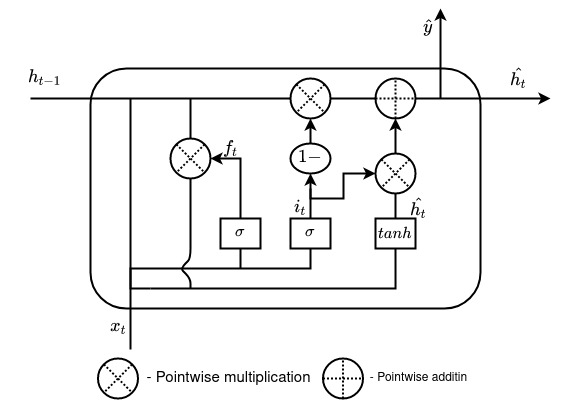
\includegraphics[width=\linewidth]{II_Body/GRU/images/GRU.jpg}
    \caption{Gated Recurrent Unit Cell}
    \label{fig:GRU-cell}
\end{figure}
\begin{equation}
    \begin{split}
        f_t &= \sigma \left (W_{f} \left [h_{t-1}, x_t \right ] + b_f \right ) \\
        i_t &= \sigma \left (W_{i} \left [h_{t-1}, x_t \right ] + b_i \right )
    \end{split}
    \label{eq:GRU-gates}
\end{equation}
%The standard activation function or content of the memory gets modified with equation~\ref{eq:GRU-output}, where \textit{func} represent the activation function and $\ast$ multiplication by element.
The memory cell output $h_t$ get calculated through the early chosen activation function, $tanh$ in \mbox{Equation~\ref{eq:GRU-output}}.
The $\ast$ stand for multiplication by element.
\begin{equation}
    \begin{split}
        \hat{h_t} &= tanh \left (W_{\hat{h}} \left [f_t \ast h_{t-1}, x_t \right ] + b_{\hat{h}} \right ) \\
        h_t &= \left (1-i_t \right ) h_{t-1}+i_t \hat{h_t}
    \end{split}
    \label{eq:GRU-output}
\end{equation}
% The GRU can act both as a stateful and stateless cell for the model by implementing the model training library.
% For comparison, a Stateful cell will be used per implementation from Song et al.~\cite{song_lithium-ion_2018} and similar articles.
%
% By implementing a model training library, the GRU can act as a stateful and stateless cell for the model.
%(1) - not even count. The method proposed by Y.Song2018, Remaining Useful Life (RUL), \textcolor{red}{uses Capacity only. Nothing more. However, no one mentioned the Statefulnes of GRU models. This would be the best place to introduce it once properly figured out.} \\[2pc]
%
%
% (3) Method proposed by B.Xiao2019 enhances GRU model training with an Ensemble optimisation method.
% Instead of utilising standard Adam optimiser, it combines Nadam and Adamax by running one after another.
% For the first 1/3 training iterations (epochs), Nadam optimiser was used for model pre-training due to its' fast converging speed, then Adamax for model fine-tuning to determine the remaining parameters. \\
% The algorithms for model fitting are as follow \\
%
%
% (8) Similar to LSTM, a Gated Recurrent Unit is intended to solve the vanishing gradient problem.
%     Unlike Chemali2017 implementation, where the training set has consisted of input data sequences with stateles model, BinXio2019 used a stateful model within batches. In addition, it introduced a technique of optimisation to the speedup training process.
%     Implementation of the model based on BinXio or someone else. Introduce their implementation and how to improve optimisation using two algorithms per their discussion.

% \subsection{Implementation}
%     Instead of implementing learning based on Battery Capacity, the following method will use the State of Charge as an input and output, similar to the Dense example. Folowing table highglights parameters, which proven to be most effective during the tests.  \textbf{Table of the parameters like BinXiao}. The activation function was selected as the \textit{tanh} \textbf{the number of sample experementaly was selected as 500?? .} \\
%     \textbf{I have found the place to describe statefulnes for the first time. Potentially, it needs to implement properly. Use the following link to understand how to keep it between batches.}
%https://machinelearningmastery.com/time-series-prediction-lstm-recurrent-neural-networks-python-keras/

